\newcommand{\obenlinks}{Software Engineering}		% hier Name der Veranstaltung eintragen
% Author: Phil Steinhorst, p.st@wwu.de
% https://github.com/phist91/latex-templates

\documentclass[%
	paper=a4,
	fontsize=10pt,
	ngerman
	]{scrartcl}

% Basics für Codierung und Sprache
% ===========================================================
	\usepackage{scrtime}
	\usepackage{etex}
	\usepackage{shellesc}					% Compiler-Option -shell-escape benutzen!
	\usepackage[final]{graphicx}			% Einbindung von Grafiken
	\usepackage[utf8]{inputenc}				% Dateien sind UTF8-codiert
	\usepackage{babel}						% deutsche Silbentrennung, etc.
	\usepackage[german=quotes]{csquotes}	% deutsche Anführungszeichen mit \enquote{...}
% ===========================================================

% Fonts und Typographie
% ===========================================================
	\usepackage{sourcecodepro}
	\usepackage[default]{sourcesanspro}
	\usepackage{nimbusmononarrow}
	
	\usepackage[babel=true,final,tracking=smallcaps]{microtype}
	\DisableLigatures{encoding = T1, family = tt* } % keine Ligaturen für Monospace-Fonts
	\usepackage{ellipsis}
% ===========================================================

% Farben
% ===========================================================
	\usepackage[usenames,x11names,final]{xcolor}
% ===========================================================

% Mathe-Pakete und -Einstellungen
% ===========================================================
	\usepackage{mathtools}					% Tools zum Setzen von Formeln
	\usepackage{amssymb}					% übliche Mathe-Symbole
	\usepackage[bigdelims]{newtxmath}		% moderne Mathe-Font
	\allowdisplaybreaks						% seitenübergreifende Rechnungen
	\usepackage{bm}							% math bold font
	\usepackage{wasysym}					% noch mehr Symbole
	\usepackage{forest}
	\usepackage{pifont}% http://ctan.org/pkg/pifont
% ===========================================================

% TikZ
% ===========================================================
	\usepackage{tikz}
	\usepackage{tikz-cd}					% kommutative Diagramme
	\usetikzlibrary{arrows.meta}			% mehr Pfeile!
	\usetikzlibrary{calc}					% TikZ kann rechnen
	\tikzset{>=Latex}						% Standard-Pfeilspitze
% ===========================================================

% Seitenlayout, Kopf-/Fußzeile
% ===========================================================
	\usepackage{scrpage2}
	\pagestyle{scrheadings}
	\usepackage[top=3cm, bottom=3cm, left=2.5cm, right=2cm]{geometry}
	\clearscrheadfoot 
	\setheadsepline{0.4pt}			 					% Linie in Kopfzeile
	\setfootsepline{0.4pt}								% Linie in Fußzeile
	\setkomafont{pagehead}{\bfseries}					% Schriftart Kopfzeile
	\setkomafont{pagefoot}{\normalfont\footnotesize}	% Schriftart Fußzeile 
	\cfoot{\thepage}									% Seitenzahl unten Mitte
	\lohead{\obenlinks}	% Titel oben links
	\raggedbottom							% Flattersatz
	\usepackage{setspace}					% erweiterte Abstandsoptionen
	\onehalfspacing							% Zeilenabstand 1.5-fach
	\setlength{\parindent}{0pt}				% Einrückung neuer Absätze
	\setlength{\parskip}{0.5\baselineskip}	% Abstand neuer Absätze
% ===========================================================

% Hyperref für Referenzen und Hyperlinks
% ===========================================================
	\usepackage[%
		hidelinks,
		pdfpagelabels,
		bookmarksopen=true,
		bookmarksnumbered=true,
		linkcolor=black,
		urlcolor=SkyBlue2,
		plainpages=false,
		pagebackref,
		citecolor=black,
		hypertexnames=true,
		pdfborderstyle={/S/U},
		linkbordercolor=SkyBlue2,
		colorlinks=false,
		backref=false]{hyperref}
	\hypersetup{final}
% ===========================================================

% Listen und Tabellen
% ===========================================================
	\usepackage{multicol}
	\usepackage[shortlabels]{enumitem}
	\setlist{itemsep=0pt}
	\setlist[enumerate]{font=\sffamily\bfseries}
	\setlist[itemize]{label=$\triangleright$}
	\usepackage{tabularx}
% ===========================================================

% listings
% ===========================================================
\usepackage{listingsutf8}
\lstset{
	belowcaptionskip=1\baselineskip,
	breaklines=true,
	showstringspaces=false,
	basicstyle=\ttfamily,
	keywordstyle=\bfseries\color{green!40!black},
	commentstyle=\itshape\color{purple!40!black},
	stringstyle=\color{orange},
	numbers=left,
	numberstyle=\footnotesize\ttfamily\color{gray},
	inputencoding=utf8/latin1,
	tabsize=4,
}

%%%%%%%%%%%%%%%%%%%%%%%%%%%%%%%%%%%%%%%%%%%%%%%%%%%%%%%%%%%
%%% Ab hier folgen nur noch vordefinierte Shortcuts %%%
%%%%%%%%%%%%%%%%%%%%%%%%%%%%%%%%%%%%%%%%%%%%%%%%%%%%%%%%%%%

\newcommand{\BB}{\mathbb{B}}
\newcommand{\CC}{\mathbb{C}}
\newcommand{\NN}{\mathbb{N}}
\newcommand{\QQ}{\mathbb{Q}}
\newcommand{\RR}{\mathbb{R}}
\newcommand{\ZZ}{\mathbb{Z}}
\newcommand{\oh}{\mathcal{O}}

\newcommand{\ol}[1]{\overline{#1}}
\newcommand{\wt}[1]{\widetilde{#1}}
\newcommand{\wh}[1]{\widehat{#1}}

\DeclareMathOperator{\id}{id} 				% Identität
\DeclareMathOperator{\pot}{\mathcal{P}}		% Potenzmenge

% Klammerungen und ähnliches
\DeclarePairedDelimiter{\absolut}{\lvert}{\rvert}		% Betrag
\DeclarePairedDelimiter{\ceiling}{\lceil}{\rceil}		% aufrunden
\DeclarePairedDelimiter{\Floor}{\lfloor}{\rfloor}		% aufrunden
\DeclarePairedDelimiter{\Norm}{\lVert}{\rVert}			% Norm
\DeclarePairedDelimiter{\sprod}{\langle}{\rangle}		% spitze Klammern
\DeclarePairedDelimiter{\enbrace}{(}{)}					% runde Klammern
\DeclarePairedDelimiter{\benbrace}{\lbrack}{\rbrack}	% eckige Klammern
\DeclarePairedDelimiter{\penbrace}{\{}{\}}				% geschweifte Klammern
\newcommand{\Underbrace}[2]{{\underbrace{#1}_{#2}}} 	% bessere Unterklammerungen
% Kurzschreibweisen für Faule und Code-Vervollständigung
\newcommand{\abs}[1]{\absolut*{#1}}
\newcommand{\ceil}[1]{\ceiling*{#1}}
\newcommand{\flo}[1]{\Floor*{#1}}
\newcommand{\no}[1]{\Norm*{#1}}
\newcommand{\sk}[1]{\sprod*{#1}}
\newcommand{\enb}[1]{\enbrace*{#1}}
\newcommand{\penb}[1]{\penbrace*{#1}}
\newcommand{\benb}[1]{\benbrace*{#1}}
\newcommand{\stack}[2]{\makebox[1cm][c]{$\stackrel{#1}{#2}$}}
\usepackage{float}

\begin{document}
	\begin{center}
		\begin{tabular}{|rlp{4cm}rll|}
		\hline
		 \textbf{Übungsblatt:} & 3 &   & \textbf{1. Abgabepartner:} & Matthias Wolff & (458 766)  \\
		        & & & \textbf{2. Abgabepartner:} & Anton Mende & (461 328) \\
		        & & & \textbf{2. Abgabepartner:} & Anika Herbermann & (461 655) \\ \hline
		\end{tabular}
	\end{center}
\section*{Aufgabe 9}
\section*{Lastenheft: Pizza-Bestellsystem der Pizzaria Vesuv}
\section{Zielbestimmung}
Die zu entwickelnde Software soll die Bestellung von Pizzen, sowie die Anmeldung und/oder Registrierung von Kunden ermöglichen.
\section{Produkteinsatz}
Das Produkt dient der Annahme von Pizza-Bestellungen. Zielgruppe des Produkts sind die Kunden der Pizzeria Vesuv.
\section{Produktübersicht}
Umweltdiagramm
\begin{figure*}[htp]
	\centering
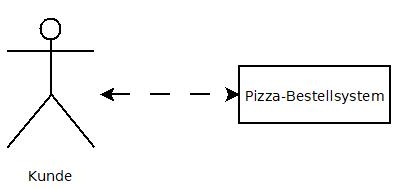
\includegraphics[keepaspectratio]{Umweltdiagramm.jpeg}
\caption {Umwelt des Produkts Pizza-Bestellsystem}
\end{figure*}
\section{Produktfunktionen}
\begin{enumerate}[/LF10/]
	\item Geschäftsprozess: Bestellung\\
	Akteur: Kunde\\
	Beschreibung: Ein Kunde wählt die für ihn relevanten Pizzen aus und gibt jeweils eine Anzahl an. Eine Anmeldung ist erforderlich.
	\item Geschäftsprozess: Anmeldung\\
	Akteur: Kunde\\
	Beschreibung: Ein Kunde meldet sich mit E-Mail und Passwort an.
	\item Geschäftsprozess: Registrierung\\
	Akteur: Kunde\\
	Beschreibung: Ein Kunde hinterlegt Name, Adresse, Telefonnummer, E-Mail-Adresse und ein Passwort.
\end{enumerate}
\section{Produktdaten}
\begin{enumerate}[/LD10/]
	\item Bestellungsdaten
	\item Kundendaten
\end{enumerate}
\section{Produktdaten}
\begin{enumerate}[/LL10/]
	\item Alle Reaktionszeiten auf Benutzereingaben müssen unter 0.5  Sekunden liegen.
\end{enumerate}
\section{Qualitätsanforderungen}
\begin{tabular}{l|cccc}
	Produktqualität&sehr gut&gut&normal&nicht relevant\\\hline
	Funktionalität&&&\texttimes&\\
	Zuverlässigkeit&&\texttimes&&\\
	Benutzbarkeit&\texttimes&&&\\
	Effizienz&&&&\texttimes\\
	Änderbarkeit&&&\texttimes&\\
	Übertragbarkeit&&&&\texttimes
\end{tabular}
\section{Ergänzungen}
keine
\section*{Glossar}
-
\section*{Aufgabe 10}
\begin{enumerate} [a)]
	\item \begin{enumerate} [1.]
		\item context Vorfuehrung \\
		inv: start <= end
		\item context Vorfuehrung\\
		inv: grundpreis > 0.0
		\item context Vorfuehrung \\
		inv: name <> “”
	\end{enumerate}
\item \phantom{a}\\
\begin{tabular}{ll}
	context Vorfuehrung&\\
	inv: Bestellung.allInstances ->&\\
	&select(b|b.Vorfuehrung = Vorfuehrung) ->\\
	&forAll(b1,b2 | b1<> b2 implies b1.reservierteSitze -> excludesAll(b2.reservierteSitze))\\
\end{tabular}
\item context Bestellung:: cancel()\\
pre: Zeitpunkt < Vorfuehrung.start
\item context Vorfuehrung \\
inv: saal.nummer = 42 implies ende < 11.11.2020
\end{enumerate}
\end{document}